\documentclass[10pt]{article}
\usepackage[final]{graphicx}
\usepackage{amsfonts}
\usepackage{amsmath}
\usepackage{caption}
\usepackage{subcaption}
\usepackage{url}
\usepackage{enumitem}
\usepackage{calc}

\topmargin-.5in
\textwidth6.6in
\textheight9in
\oddsidemargin0in

\def\ds{\displaystyle}
\def\d{\partial}

\begin{document}

\centerline{\large \bf Given a helical compression spring in a spring-mass-damper system, what are optimal springs?}

\vspace{.1truein}

\def\thefootnote{\arabic{footnote}}
\begin{center}
  
  Alistair Bentley\footnote{Mathematics, Clemson University},
   Tim Hodges\footnote{Mathematics, Colorado State University},
   Jiahua Jiang\footnote{Mathematics, University of Massachusetts Dartmouth },
  Justin Krueger\footnote{Mathematics, Virginia Tech},
  Saideep Nannapaneni\footnote{Civil \& Environmental Engineering,Vanderbilt University},
  Tianyu Qiu\footnote{Mathematics, University of Delaware}
   
\end{center}


%\vspace{.1truein}

\begin{center}
Problem Presenters: Jordan Massad\footnote{Sandia National Laboratory},
Sean Webb\footnote{Sandia National Laboratory};
	Faculty Mentors: Ilse Ipsen\footnote{Mathematics, North Carolina State University},
	Ralph Smith\footnote{Mathematics, North Carolina State University}, 
\end{center}


\vspace{.3truein}
\centerline{\bf Abstract}





\section{Introduction}
\label{sec:Introduction}
%It should be written as much as possible in non-technical terms, so that a
%lay reader can understand the context and the contribution of the paper.

% Fix long sentence remove figure
Springs have many everyday uses, and scientists have studied them thoroughly as a result~\cite{Wahl}. We find them in cars, homes, gyms, and industry, and one common use of helical compression springs, in particular, is in mechanical switches~\cite{SpringDevice}. Acceleration switches, such as the one seen in Figure~\ref{Acceleration Switch}, are used to close electrical circuits once the object carrying the switch reaches a certain acceleration. The main use of such switches is to provide power to sensory equipment and data recorders for very precise amounts of time, and one example of their use is collecting data from rocket sled experiments. 

		\begin{figure}[h]
		 \begin{center}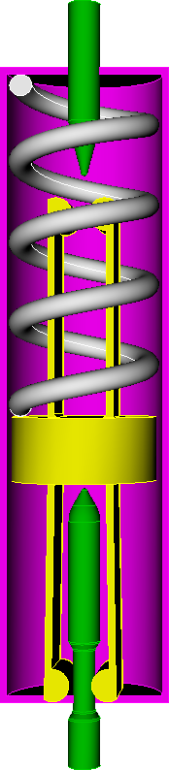
\includegraphics[scale=.2]{Acceleration_Switch.png}\end{center}
		 \caption{An example of an acceleration switch, see reference \cite{Massad2015}.}
		 \label{Acceleration Switch}
		 
		 \end{figure}	 
		
These rocket sled tests include very high velocities and accelerations and end in a destructive impact, and since the test is not easily replicated, we must have the ability to consistently and correctly collect data. This means we require that the spring in the acceleration switch must behave as expected to the forces exerted on it, and having a switch that is closed earlier or later than expected is undesirable~\cite{IMSM2010}. Designing a spring to behave as desired is a complicated problem that requires satisfying numerous constraints on the spring's physical properties. That the desired spring can vary depending on the application further complicates the problem. 

Spring design under these conditions amounts to a constrained optimization problem where certain properties of the spring may need to be maximized or minimized subject to bounds on some or all of the spring's other properties. Extending the scope of focus beyond springs' use in mechanical switches, which already cover a vast spread of specific spring designs, results in even more possibilities for design specifications. Rather than developing methods to solve these problems on an ad hoc basis, developing tools to address a wide variety of constrained optimization problem formulations for spring design would be beneficial. 

Designing an optimal spring is not a new problem. Brake et al. considered the design of an acceleration switch with enabled uncertainty~\cite{IMSM2010}. Alternatively, Sastry et al. implemented probabilistic response surface methodology to investigate the complications of uncertainty in designing a spring~\cite{Reliability}. Others have considered the reduction of the optimization problem to focus on a single parameter~\cite{Robust}. Similar tools to the ones mentioned above also exist~\cite{Paredes}.

Motivated by the premise of the workflow shown in Figure~\ref{Workflow}, we produce a novel tool with new capabilities. 

		\begin{figure}[h!]
		 \begin{center}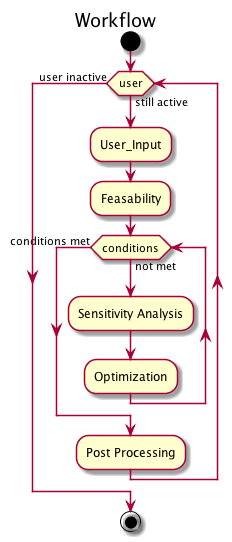
\includegraphics[scale=.4]{IMSM_Workflow.png}\end{center}
		 \caption{Illustration of the flow of our approach.}
		 \label{Workflow}
		 
		 \end{figure}
		 
The novelties we include are the inherit flexibility in our tool's framework, tools to visualize the existence of solutions for constrained optimization problems, sensitivity analysis capabilities, and design optimization under uncertainty. We also discuss the inclusion of stress relaxation constraints in the spring design, which to our knowledge has not been considered before. We provide details regarding these items as follows. Section~\ref{sec:The_Problem} formally defines the spring design problem for helical compression springs. Section~\ref{sec:The_Approach} expands on the workflow shown in Figure~\ref{Workflow}. Section~\ref{Computational_Experiments} shares cases studies using our approach, and Section~\ref{Summary} summarizes our work and provides suggestions for future work.


%%For this example we must optimize the spring to give the best chances of success. Velocities of a rocket sled may vary depending on application, so we should be able to optimize the spring for the application. This leads to an optimization problem. The problem is well defined once the constraints are understood and the objective function that must be maximized or minimized is defined. 
%
%\subsection{Generalizing The Example}
%Expanding on the scope of this problem, a switch may be used in a myriad of ways \cite{SpringDevice}. Depending on the application it is important that one can find an optimal spring. The optimization problem must now require flexibility to allow how a spring is determined to be optimal. In other words, there can be a variety of objective functions and a variety of constraints that are possible.   
%
%For any set of constraints and objective function the optimization problem will depend on a set of variables. In optimization we only wish to concern ourselves with the variables for optimization. One can implement structures to hold all data for a spring, and access the relevant  variables for optimization when needed. 
%
%In addition, with the expansion of the problem comes the growth of uncertainty in the problem. One can quantify the uncertainty of the problem by conducting a sensitivity analysis of the objective function subject to the constraints and variables given. 
%\newline
%
%The problems that will be discussed in this paper are as follows: 
%\begin{itemize}
%	\item Can we develop a flexible framework for designing an optimal spring?
%
%	\item Is one able to incorporate feasibility?
%	
%	\item What about the concept of stress relaxation?
%	
%	\item What about uncertainty in design optimization? 
%	
%	
%\end{itemize}

%\subsection{History}
%Designing an optimal spring is not a new problem. In 2010 at the SAMSI IMSM workshop a team considered the design of an acceleration switch with enabled uncertainty. In fact, the switch they considered was in figure \ref{Acceleration Switch}. This approach lead to a paper \cite{IMSM2010}. This is not the only approach to uncertainty, in \cite{Reliability} probabilistic response surface methodology was implemented to investigate the complications of uncertainty in designing a spring. In addition to these types of approaches it is possible to narrow focus to a single parameter, in \cite{Robust} they focus on the spring stiffness. In \cite{Paredes} they attempt to design an optimal spring, with the introduction of a sizing tool. All references listed are informed to some extent by \cite{Wahl}. 




%In this paper we will give a description of the springs of interest, helical compression springs, see section \ref{sec:Springs}. Next, the formulation of the problem, see section \ref{sec:Problem}, and the approach taken to the problem see section \ref{sec:Approach}. Following will be a section on workflow with descriptions of each step in the workflow see \ref{sec:workflow}. We will discuss a few case studies given the framework constructed, see \ref{sec:Experiments}. Lastly, a summary with future work that can be worked on, see \ref{sec:summary}.





\section{Helical Compression Springs}
\label{sec:Springs}

Helical springs are the typical spring that comes to most peoples mind, for illustrative purposes, see figure \ref{Spring}. 

		\begin{figure}[h]
		 \begin{center}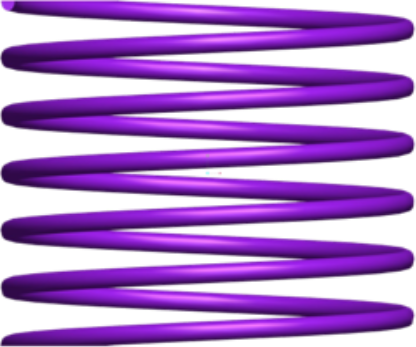
\includegraphics[scale=.2]{Spring.png}\end{center}
		 \caption{An example of a helical compression spring, from \cite{Massad2015}}
		 \label{Spring}
		 
		 \end{figure}

The above spring has many design parameters. These range from physical parameters such as wire diameter, to purely empirical attributes. The empirical attributes have to be assumed in a range of values. If they are not extreme values will exhibit behavior we do not wish to consider. Below is a list of a spring's key design parameters and empirical attributes. We have added a few figures to illustrate some of the parameters. \cite{Massad2015}		 
		\begin{figure}[h]
			\centering
			\begin{subfigure}{.5\textwidth}
				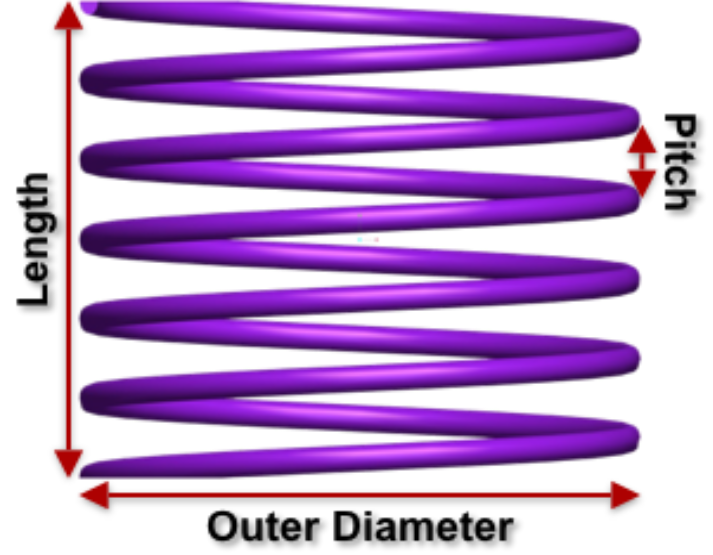
\includegraphics[scale=.2]{Spring_Description.png}
				\caption{Pitch, outer diameter, and length of a spring.}
				\label{Description1}
			\end{subfigure}%
			\begin{subfigure}{.5\textwidth}
				  \centering
		 		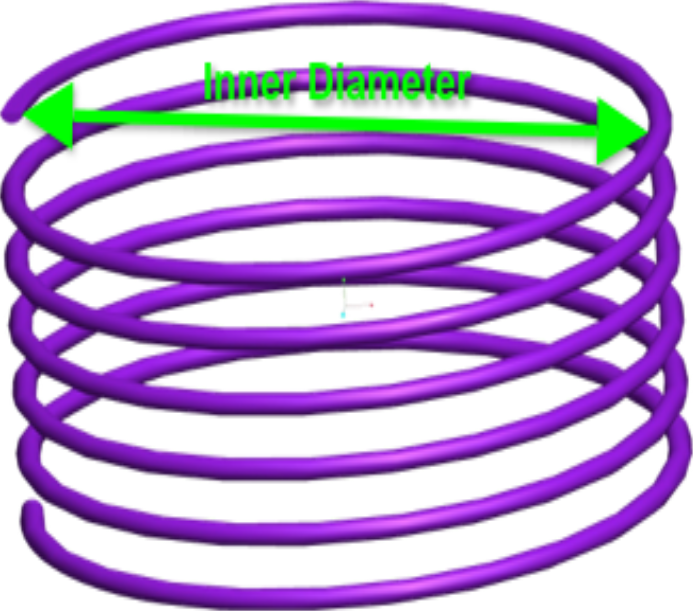
\includegraphics[scale=.2]{Spring_Description2.png}
				\caption{Inner diameter}
				  \label{Description2}
		  		
			\end{subfigure}
			 \label{Descriptions}
		  \caption{A few figures that show some parameters for a helical compression spring.}
		\end{figure}
		
		% Group parameters and change from enumerate
		\noindent \textbf{Parameters:}
		\begin{description}[leftmargin=!,labelwidth=\widthof{\bfseries Outer diameter:}]
			\item [Inner diameter:] denoted $\mathbf{d_{i}}$, illustrated in figure \ref{Description2}.
			
			\item [Outer diameter:] denoted $\mathbf{d_{o}}$, illustrated in figure \ref{Description1}.
			
			\item [Wire diameter:] denoted $\mathbf{d_{w}}$.
			
			\item[Total coils:] denoted $\mathbf{N_{t}}$, this is the number to rotations of wire in the spring, we allow for partial rotations.
			
			\item[Active coils:] denoted $\mathbf{N_{a}}$, active coils are not touching any other coils. The number of active coils is subject to the spring being closed or open. Closed means that the end coils are welded, where as open means they are not. For this reason a spring must have at least 2 coils.

			\item[Free length:] denoted $\mathbf{L_{free}}$, the spring's length without any force applied. i.e., this is the spring length before being installed in the acceleration switch.
			
			\item[Solid length:] denoted $\mathbf{L_{solid}}$, the spring's length when all coils are compressed together.
			\item[Open length:] denoted $\mathbf{L_{open}}$, the spring's length at open position. i.e., for the acceleration switch this would be before the rocket sled test is started. 
			
			\item[Close length:] denoted $\mathbf{L_{close}}$, spring length at close position. i.e., this would be when enough force is applied for the acceleration switch to close and start collecting data.
			
			\item[Hard length:] denoted $\mathbf{L_{hard}}$, the maximum a spring can compress for the application. i.e., for the acceleration switch this is the maximum compression the acceleration switch's spring should be allowed. 
			
			\item[Open force:] denoted $\mathbf{F_{open}}$, this is the force on the spring in open position, i.e., the resting force for the acceleration switch.			
			
			\item[Pitch:] denoted $\mathbf{p}$ illustrated in figure \ref{Description1}, depends on the $\mathbf{d_{w}}$,$\mathbf{L_{free}}$, and $\mathbf{N_{a}}$.t			
			
			\item[Shear modulus:] (or modulus of rigidity), denoted $\mathbf{G}$, is one of several quantities for measuring the stiffness of materials.
			
			\item[Young's modulus:] (or elastic modulus), denoted $\mathbf{E}$, is a measurement of force that is needed  to stretch (or compress) a sample of material.
			
			\item[Poisson ratio:] denoted $\mathbf{\nu}$, is a measurement of the poisson effect of a material. 
			
			\item[Ultimate torsional stress:], denoted $\mathbf{UTS}$. 
		
		\end{description}

% Give context to statement		
One can see that the above parameters are physical design parameters. Each of these are subject to design tolerances. Below is a set of empirical attributes that within a range of values exhibit typical behavior for a spring. We will assume that these attributes are within that range. 
			
			\begin{description}
				\item [Spring Rate (k):] \begin{equation} k = \frac{G}{8N_{a}}\frac{d_{w}^{4}}{(d_{i} + d_{w})^{3}}\end{equation}
				\end{description}
			The spring rate is a quantity used to measure the rigidity or stiffness of the object. 
			\begin{description}	
			\item[Spring Index (C):]\begin{equation}C = \frac{d_{i}}{d_{w}} + 1.\end{equation}
			\end{description}
				 The spring index gives a measurement of the inner diameter to the wire diameter. This is useful because outside of certain values the design will require more tolerance and cost also increases. \cite{SpringIndex}
			\begin{description}	
			\item[Coil Binding Gap:]\begin{equation} g = \frac{L_{hard} - L_{solid}(d_{w},N_{a}; ec)}{N_{t} - 1}\end{equation}
			\end{description}
				If the spring is allowed to go to solid compression, it is possible the spring could continue compression and cause coils to bind. Think about your favorite slinky. $L_{solid}$, is in terms of $d_{w}$, $N_{a}$, and end conditions (ec). Refer back to $N_{a}$ for what end conditions mean physically.
		

		\begin{description}
			 \item[Max Shear Stress:]\begin{equation} \frac{G(L_{free} - L_{hard})}{4 \pi N_{a} (ec)} \left[\frac{d_{w} (4d_{i}^{2} + 9.46d_{i} 
d_{w} + 3 d_{w}^{2})}{d_{i}(d_{i}+d_{w})^{3}}\right]< UTS\end{equation}
		\end{description}
				Shear stress is a measurement of stress coplanar to the spring, this puts a maximum we allow. 
			\begin{description}
			\item[Diametral Expansion($d_{expand}$):]\begin{equation} d_{expand} = d_{w} + \sqrt{(d_{i} + d_{w})^{2} + \frac{p^{2} - d_{w}}{\pi^{2}}}
			\end{equation}
			\end{description}
			This is the expansion of the diameter as compression of the spring is happening. One may notice that \begin{equation}p^{2} \ge d_{w} - \pi^{2} (d_{i} + d_{w})^{2},\end{equation} this is putting an implicit constraint on how much the spring can be extended/compressed.
			



			
			
\section{The Problem} 
\label{sec:The_Problem}

\textbf{Add dependency graph.} 

Design an algorithm that optimizes springs with interchangeable objectives and constraints. In addition, attempt to incorporate properties stress relaxation and creep into the available objectives and constraints. 

A list of possible constraints/objectives given in minimization form is below, please note that \\$d_{i}^{max}, d_{o}^{max}, k_{max}, C_{max}$, and $g_{min}$ are user defined bounds. 
 % remove repetitions
\begin{enumerate}
	\item $d_{i} < d_{i}^{max}$, this sets a design constraint on what we will allow the inner diamter to be. For the acceleration switch, we must have a spring that will fit the housing of the switch.
	\item $d_{i} < d_{o}$, physically we must have a bigger outer diameter than inner diameter.
	\item $d_{i} + 2d_{w} < d_{o}^{max}$, The outer diameter cannot exceed some design limitation.
	\item$d_{expand} - d_{0}^{max} < 0 $, we will not allow the spring to expand more than a certain amount during compression.
	\item$ \frac{G}{8N_{a}}\frac{d_{w}^{4}}{(d_{i} + d_{w})^{3}} - k_{max} \le 0 $, there is a maximum spring rate or stiffness that we will allow. 

	\item $\frac{d_{i}}{d_{w}} + 1 - C_{max}< 0$, similarly we will only allow a maximum ratio between the inner diameter and wire diameter. 

	\item $(L_{free} - L_{open})\frac{G}{8N_{a}}\frac{d_{w}^{4}}{(d_{i} + d_{w})^{3}} - F_{open} = 0 $, $F_{open}$ should be physically possible given its formulation.

	\item $\frac{L_{hard} - L_{solid}}{N_{t} - 1} + g_{min} \le  0$. There is a minimum gap we wish to have to ensure our coils cannot bind. 

	\item$\frac{L_{free}}{d_{i} + d_{w}} - \pi \sqrt{\frac{2(2 \nu + 1)}{\nu + 2}}$, if a spring is slender, it may buckle or fold on itself. This is a constraint to address this physical attribute. 

	\item$-UTS + \frac{G(L_{free} - L_{hard})}{4 \pi N_{a} (ec)} \left[\frac{d_{w} (4d_{i}^{2} + 9.46d_{i} 
d_{w} + 3 d_{w}^{2})}{d_{i}(d_{i}+d_{w})^{3}}\right] < 0$

We do not wish to allow the torsional stress to exceed a certain amount, the ultimate torsional stress, $UTS$.

\end{enumerate}	

% remove the extra specifics
This list is not exhaustive as we want a user to be able to define new constraints and objectives. The incorporation of stress relaxation and creep are two examples of this. If the reader wishes to read about these in detail please check out section \ref{sec:stress}. 

In addition to these we should be able to minimize any parameter of the spring. It may be possible they wish to minimize the wire diameter, or the length of the spring at a certain state.  

In order to simplify the problem we have some assumptions. First, we have assumed that constraints and objectives are all in terms of the number of total coils. This is to reduce the complexity of knowing if a constraint is dependent on the active number or total number of coils. These two numbers are dependent on the end conditions of the spring, whether it is open or closed at the end. 

For this reason we also will consider all springs to be have a closed end condition. With these assumptions we simplify our constraints for pitch, $p$, solid length, $L_{solid}$, and the diametral expansion, $d_{expand}$.

\textbf{JUSTIFY ASSUMPTIONS}
These assumptions have reduced the set of design parameters and have allowed us to simplify the problem. Without these assumptions we would need to deduce at run time what formulas we can use and this is a challenging problem from an implementation stand point. Also, we have a very complicated formula for diametral expansion if the end conditions are not closed. This presents issues of solving a cubic without the ability of discerning if the roots will be physically meaningful. 


\subsection{Mathematical Model}
			
			The mathematical model is as follows: 
				\begin{equation*}
 					\begin{aligned}
 						& \underset{\textbf{x}}{\text{minimize/maximize}}
 						& & O(\textbf{x}) \\
 						& \text{subject to}
 						& & C(\textbf{x}) \le \textbf{y}
 					\end{aligned}
				\end{equation*}

\begin{itemize}
	\item \textbf{x} is a set of variables for optimization, they are user specified.
	
	\item \textbf{y} is a set of bounds on the constraints, they are user specified.
	
	\item O(\textbf{x}) is the objective function. It is comprised of any parameters or attributes described above. It can also include other user defined attributes and parameters not considered in this paper. The user specifies the objective function.  
	
	\item C(\textbf{x}) is the list of constraints. It is comprised of any parameters or attributes described above. It can also include other user defined attributes and parameters not considered in this paper. The user specifies the constraints to use.
\end{itemize}

% pull top stuff down into sections

\section{The Approach}
\label{sec:The_Approach}

\textbf{Present and justify approach for solving the problem}
\textbf{Explain advantages of approach over existing ones}
\textbf{Tell a story}
To be as flexible as possible we must be able to handle constraints and objectives that have an unknown number of  variables a priori. To handle this uncertainty we instead of evaluating an objective or constraint with a set of values we evaluate with a "spring object" in the programming sense \cite{OOP}. This spring has all the attributes of interest and the function merely picks what values it needs for evaluation. 

This approach is also implemented in the design of a constraint and objective. An objective is an expression that we must be able to evaluate. A constraint is an expression that we must evaluate and check if this evaluation violates the constraint condition. We use the idea of inheritance and let a constraint inherit the properties of being an objective with additional framework to compare to a condition. This allows the user to interchange constraints and objectives seamlessly.

Along with the flexible software design, we have implemented the ability to run feasibility and sensitivity checks before trying to optimize. This will allow the user to know additional information about the problem. First, from feasibility, the user will know quickly if the run is unable to find a feasible point to run optimization. Second, from sensitivity, the user can know which parameters will dramatically change the optimization versus which parameters are unnecessarily adding to the dimension of the optimization space. 
 


\section{Workflow}
\label{sec:workflow}
 		\begin{figure}[h!]
		 \begin{center}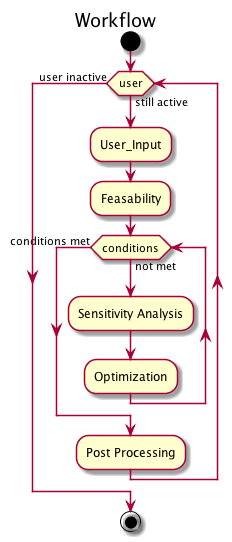
\includegraphics[scale=.6]{IMSM_Workflow.png}\end{center}
		 \caption{Illustration of the flow of our approach.}
		 \label{Workflow}
		 
		 \end{figure}
		 
		 \textbf{This may not be accurate anymore, need Justin's input.}
Above is an illustration of the workflow that is our approach. This section will go in depth into the feasibility, sensitivity analysis and optimization of our approach.

\textbf{Should we add a workflow of feasibility, sensitivity, and optimization?}

\subsection{User Input}
\section{User Input}

The first step in our work flow is receiving an arbitrary optimization problem from the user.  In general, this includes an optimization function, a list of free variables and a set of constraints.  From a practical standpoint, it is not feasible to build an algorithm that handles such a large set of problems.  Thus, the first task in our work flow is to maximize the user's ability to specify a problem while still being able to generate a meaningful solution.  As a solution, we place some limits the user's input and designed a program capable of solving this restricted class of problems.

To reduce the size of the permissible problem space, two restrictions are put on the user's input problem.  First, the user must specify the optimization function as a weighted sum of minimums and maximums.  While other methods for multicriteria optimization exist, implementing these into our scheme has been left to future work.  Second, based on discussions with engineers experienced with spring design, we restricted the space of free variables to those that are considered most important.

Next, to allow our program to handle any problem formulated on this reduced problem space, our software uses an object oriented design.  Object-oriented programming is an approach to software design that centers around classes.  Classes are essentially data containers capable of performing a predefined set of tasks.  For example, our program uses a \textbf{constraint} class that includes the constraint's function, and a way to check whether the constraint is violated at a given point.

Using classes allow flexibility because the program's algorithm can be designed to operate on the classes.  For example, the \textbf{OptimizationProblem} class generates the input for the optimizer and sensitivity analysis.  Thus when the user inputs a new problem, the program generates an \textbf{OptimizationProblem} with a specific optimization function and set of constraints.  Thus, the final stage of the user input process is translating the set of optimization parameters into instances of the program's classes.

Additional points to consider...adding new constraint functions and the predefined constraints list.

% Check capitalization
\subsection{Feasibility}
\label{sec:Feasibility}

Once the user has set a problem, the next step is determining the nature of the feasible region.  To assess feasibility, we use a Latin Hypercube sampling method.  In Latin Hypercube sampling, the samples are designed to cover the entire domain.  This approach is used because the user defined constraints can be of a general nature (for example, linear or non-linear).  If a feasible point cannot be identified, the algorithm will terminate and the user is informed a feasible point cannot be found.  At this point, the user can try a more exhaustive search or reformulate the problem.

Additionally, a graphical tool has been added to help the user analyze the problem's feasible region.  As illustrated in figure-xx, a plot with two or three state variables can be displayed that highlights the problem's overall feasible region and the contributions from each individual constraint.  This will allow the user to see which constraints are most restrictive in the context of their problem.


The feasibility of a solution depends on if a solution satisfies all the constraints in the problem, as well as, constraints that are not included. We also need a feasible solution to start the optimization process, otherwise we may never find an solution that is feasible and optimal. Implementing this requirement is simply sampling the available space and checking each sample against all constraints. 

Refer to section \ref{sec:Experiments} to see plots that are showing feasibility given two or three state variables.

\subsection{Sensitivity Analysis}
\label{sec:Sensitivity}
\hspace{5 mm} As the dimension of design variable space increases, the computational expense of the optimization procedure increases. To reduce the computational expense, it is often desirable to reduce the design variable space by removing the variables that have very little influence on the objective function. Thus, a dimension reduction strategy is required to reduce the design variable space. 

Dimension reduction approaches have been divided into two categories - (1)filter approach, and (2)wrapper approach. In the filter approach, the input variables are ranked according to a ranking criterion and the most dominant variables can be selected by assuming a threshold influence value. In the wrapper approach, a subset of variables is selected from the list of all possible subsets of the input variables that best estimate the output variable. Sensitivity analysis, a filter approach, is used in this work for dimension reduction. 

Two types of sensitivity analysis have been developed in the literature - local sensitivity analysis and global sensitivity analysis. The local sensitivity index of a variable measures the sensitivity of the model output when the variable is fixed at a single value whereas the global sensitivity (GSA) index measures the variation of model output when the variable is varied over its range. Therefore, GSA is used as it considers the entire range of a variable in computing the sensitivity to the output. Note that the input variables represent the design variables and model represents the objective function.
Consider a objective function, $G$, with $n$ design variables given by $x_{1}$, $x_{2}$, ...  $x_{n}$, given by

\centerline{$Y = G(x_{1}, x_{2}, ... x_{n})$}

In GSA, two types of indices can be calculated for each variable - first order index and total effects index. The first-order index ($S_{i}^{I}$) quantifies the uncertainty contribution of an input variable, without considering its interactions with other variables, to the output variable uncertainty. Similarly, the total effects index ($S_{i}^{T}$) quantifies the uncertainty contribution of an input variable by considering its interactions with all variables, to the output uncertainty. The expressions for the two sensitivity indices are given below as 

\centerline{$S_{i}^{I} = \frac{V_{X_i}(E_{X_{-i}}(Y|X_{i}))}{V(Y)}$}
\centerline{$S_{i}^{T} = \frac{E_{X_{-i}}(V_{X_{i}}(Y|X_{-i}))}{V(Y)}$}

Given a design range (lower and upper bounds), a variable can be assumed to be uniformly distributed in the design range. For each variable, the first-order index is calculated and if it is less than an assumed threshold value, then that variable is assumed insensitive and removed from the optimization procedure. Thus, dimension reduction is implemented for a faster design optimization.\cite{Bioinformatics} \cite{Wrappers} \cite{Error} \cite{Global}


\subsection{Optimization}
\label{sec:Optimization}
\hspace{5 mm} A general constrained design optimization problem can be formulated as follows

\centerline{$Min \hspace{2 mm} f(X)$}
such that

\centerline{$g(X) \leq 0$}
\centerline{$lb_{X} \leq X \leq ub_{X}$}

\noindent Several optimization algorithms (both local and global) are available to solve the above optimization problem. Two algorithms - BFGS (local) and DIRECT (global) have been tried for design optimization. The key differences between the two algorithms are described below. BFGS algorithm requires the gradient and Hessian of the objective function, and also an initial point for optimization whereas DIRECT does not require the objective function to be differentiable. Since DIRECT is a global algorithm, it does not require an initial point. A downside of DIRECT is that it requires more computations compared to BFGS. The 'fmincon' function in MATLAB, which implements the BFGS algorithm, requires the linear and non-linear constraints to be provided separately. Separation of linear and non-linear constraints is hard to implements in an automated software framework because they are problem-dependent whereas DIRECT does not require such segregation between constraints. Therefore, DIRECT global algorithm is used for optimization.

% new subsection

\hspace{5 mm} It is also essential to account for the variability in the manufacturing process(tolerance) in the design of springs. The tolerance for each of the spring parameters is assumed to be equal to one percent of the value of the variable. Thus, each variable follows a uniform distribution with unknown mean and known variance. The optimization formulation after accounting for tolerances can now be written as 

\centerline{$Min \hspace{2mm} \mu_{f} (X,d)$}

such that

\centerline{$Pr(g_{i}(X,d) \leq 0)\geq p_{t}^{i}$}
\centerline{$Pr(X \geq lb_{X})\geq p_{lb}$}
\centerline{$Pr(X \leq ub_{X})\geq p_{ub}$}
\centerline{$lb_{d} \leq d \leq ub_{d}$}

\noindent where $X,d$ represent the design variables with tolerances and non-design variables with tolerances respectively. The first constraint represents the probabilistic inequality constraint and the other constraints represent the bounds for the design variables. Optimization with tolerance is a nested double loop process where optimization is carried out in the outer loop (using DIRECT)and in each iteration of optimization, reliability analysis is carried out in the inner loop to check the probabilistic constraints. In this work, Monte Carlo simulations are used to carry out reliability analysis. 

\cite{Derivative} \cite{DirectPaper} \cite{MATLAB:2014a} \cite{DirectUserGuide}
 
 

\section{Computational Experiments}
\label{sec:Computational_Experiments}

\newpage
\subsection{Case 1:}
\label{sec:Case1}
%Case_56_28910
	\textbf{Objectives:} Minimize spring rate and spring index.\\
	\textbf{Constraints:} Inner diameter and outer diameter relation, elation on inner, wire, and outer diameter, coil binding gap, buckling slenderness, and maximum shear stress. \\
	\textbf{State Variables:} $d_{i}$, $d_{w}$, and $N_{t}$ \\

\newpage
\subsection{Case 2:}
\label{sec:Case2}
%Case_56_34891011

	\textbf{Objectives:} Minimize spring rate and spring index.\\
	\textbf{Constraints:} Relation on inner, wire, and outer diameter, diametral expansion, coil binding gap, buckling slenderness, and maximum shear stress, stress relaxation. \\
	\textbf{State Variables:} $d_{i}$, $d_{w}$, and $N_{t}$ \\

\newpage
\subsection{Case 3:}
\label{sec:Case3}
%Case_7_348910
	\textbf{Objectives:} Minimize force at open position.\\
	\textbf{Constraints:} Relation on inner, wire, and outer diameter, diametral expansion, coil binding gap, buckling slenderness, and maximum shear stress. \\
	\textbf{State Variables:} $d_{i}$, $d_{w}$, and $N_{t}$ \\

\newpage
\subsection{Case 4:}
\label{sec:Case4} 
%Case_11_348

	
	\textbf{Objectives:} Maximize stress relaxation\\
	\textbf{Constraints:} Relation on inner, wire, and outer diameter, diametral expansion, and coil binding gap. \\
	\textbf{State Variables:} $d_{i}$, $d_{w}$, and $N_{t}$ \\



		\begin{figure}[h]
		 \begin{center}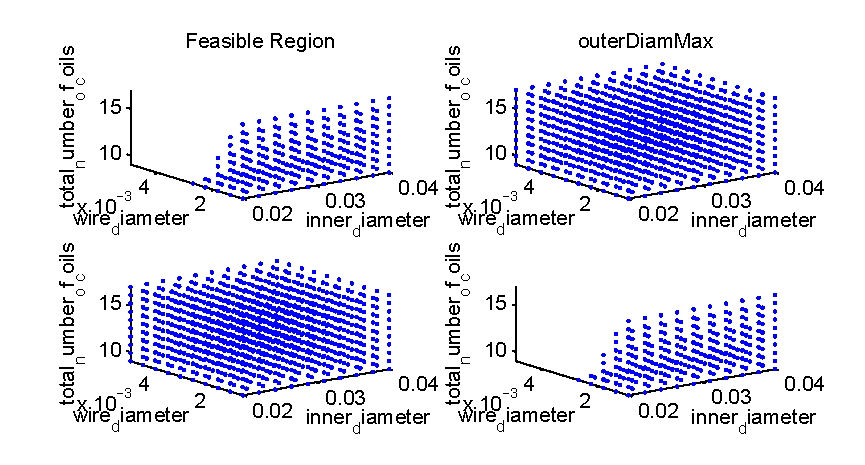
\includegraphics[scale=.75]{Case_11_348.eps}\end{center}
		 \caption{Feasible region for case 4.}
		 \label{Feasible Case 4}
		 
		 \end{figure}
 		\textbf{Axes need to be worked on.}

\newpage
\subsection{Case 5:}
\label{sec:Case5}
%Case_511_34810

	\textbf{Objectives:} Minimize spring rate and maximize stress relaxation.\\
	\textbf{Constraints:}  Relation on inner, wire, and outer diameter, diametral expansion, coil binding gap, and maximum shear stress. \\
		\textbf{State Variables:} $d_{i}$, $d_{w}$, and $N_{t}$ \\
		
				\begin{figure}[h!]
		 \begin{center}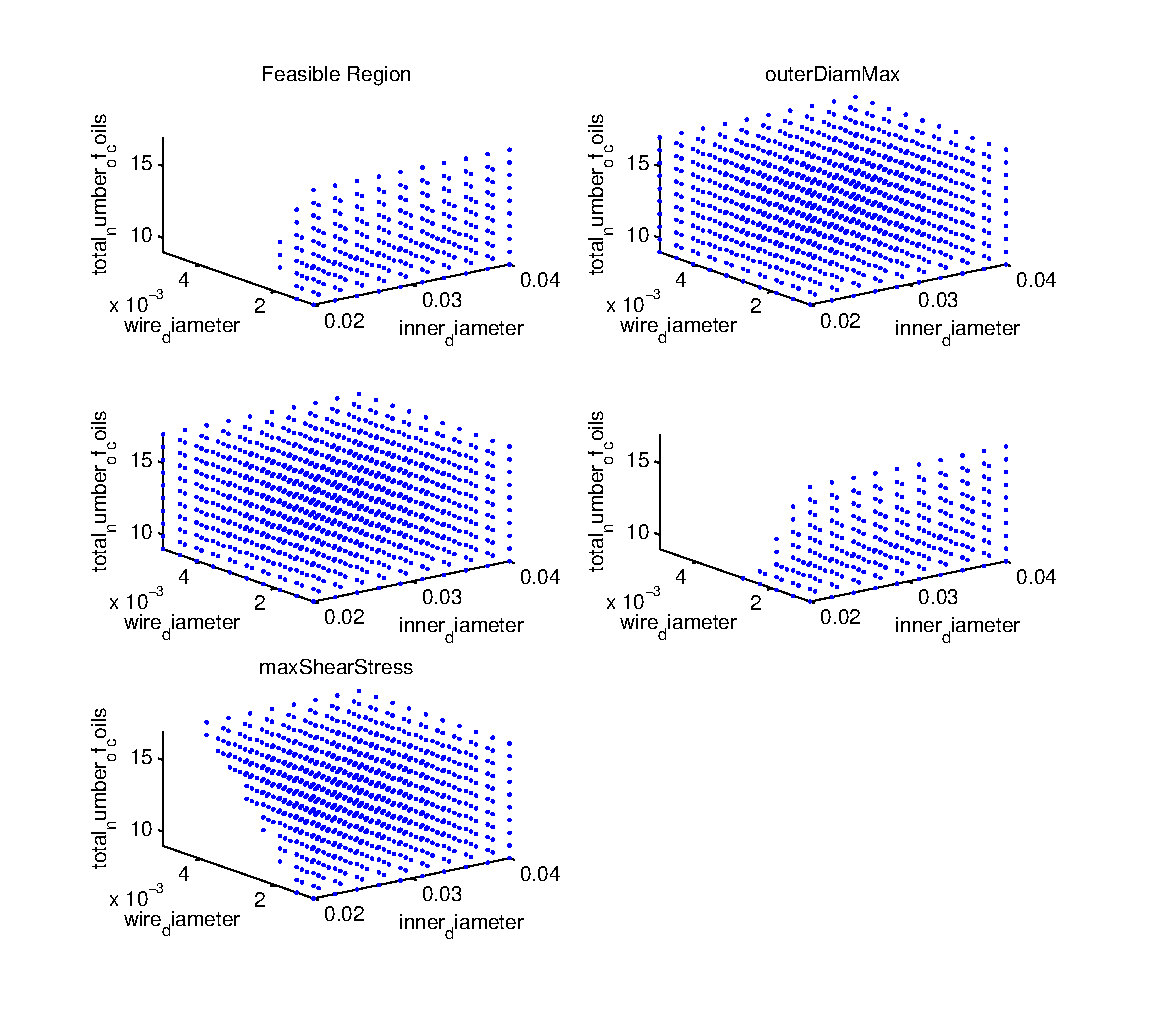
\includegraphics[scale=.50]{Case_511_34810.eps}\end{center}
		 \caption{Feasible region for case 5}
		 \label{Feasible Case 5}
		 
		 \end{figure}
		 \textbf{Axes need to be worked on.}

\newpage
\subsection{Case 6:}
\label{sec:Case6}
%Case_58_3468910
\textbf{Saideep added a 7a, need to deal with it.}\\
	\textbf{Objectives:} Minimize spring rate and coil binding gap.\\
	\textbf{Constraints:} Relation on inner, wire, and outer diameter, diametral expansion, coil binding gap, buckling slenderness, and maximum shear stress. \\
		\textbf{State Variables:}$d_{i}$, $d_{w}$, $L_{hard}$, and $N_{t}$ \\

\newpage





\section{Summary and Future Work}
\label{sec:Summary}
The ability to interchange constraints and objective functions with any number of design variables allows the user the utmost flexibility. With the addition of feasibility and sensitivity analysis it is possible for any configuration of objective function, constraints, and design variables to be analyzed for refinement. The quantification of stress relaxation and creep allow the user a chance to incorporate these properties into any configuration, especially those that have never been tested. 

Some limitations of the approach outlined are as follows. The choice of optimization and sensitivity analysis are fixed, however, they are modularized to allow a different optimization routine and sensitivity analysis to be ported in. Given the amount of flexibility that is enabled, a user will have to be able to decide if a infeasible solution is due to user error. 

Future work is bountiful for this approach. More analysis of the stress relaxation and creep could result in better performance. An in depth analysis of different models of stress relaxation and their performance in our model would be beneficial. The flexibility allows the inclusion of many different models of stress relaxation and creep to be added

\textbf{Senstivity for optimization}


\textbf{Uncertainty Quantification incorporation into the model.}



\subsection{Basics about creep and stress relaxation}
\label{sec:stress}
A rocket mounted spring is expected to deliver normal mechanical output under extreme temperatures. The analysis of creep behavior helps us design a spring to meet the requirements under rough conditions.

Creep is the strain increase under constant stress, usually activated by high temperatures. Three mechanisms have been proposed to account for the phenomenon: dislocation slip and climb, grain boundary sliding and diffusional flow. We focus on the creep caused by the dislocation mechanism. The material's creep tendency is determined by a creep test. During a test, the spring is kept at $0.3-0.5T_m$ ($T_m$ is the melting temperature of the material) and loaded by a constant tensile force.

Conventionally, creep can be divded into $3$ stages. In the first stage (primary/ reduced/trasient) ,the creep strain rate decreases to a certain value(minimum creep rate). The second stage(secondary/steady/stationary creep) is characterized by a nearly constant creep rate(minimum creep rate). In the third stage(tertiary creep), the creep strain rates increases rapidly and leads to rupture. The first stage is usually reversible with time after unloading, while the second/third ones are not. Since the primary creep occurs in a short duration and the tertiary one leads quickly to rupture, the secondary creep is under most serious consideration in many engineering designs.

Another common test to determine the material's susceptibility to high temperature is called stress relaxation. During the test the load is continuously decreased in such a way that the initial strain remains constant. The mechanism is more or less the same as that of creep.

\subsection{Creep rate law of material}
\label{sec:Creep}
The starting point is the assumption that the creep rate may be described as a product of three separate functions of stress, temperature and time
\[
\epsilon_{cr}(\sigma,T,t)=f_\sigma (\sigma) f_T(T) f_t(t)
\]
The widely used functions of stress $f_\sigma(\sigma)$ are (\cite{NaKo2006}):

\begin{tabular}{ll}
$a\sigma^n$ & Norton, 1929, Bailey, 1929 \\
$b\left( \exp{\sigma\over \sigma_0} -1 \right)$ & Soderberg, 1936 \\
$a\mathop{sinh}{\sigma\over \sigma_0}$ & Prandtl, 1928, Nadai, 1938, McVetty, 1943\\
$a_1\sigma^{n_1} + a_2 \sigma^{n_2}$ & Johnson et al., 1963 \\
$a\mathop{sinh} \left( {\sigma\over \sigma_0}\right)^n$ & Garofalo, 1965
\end{tabular}

where $a,b,a_1,a_2,\sigma_0,n_1,n_2$ are material constant. The dependence on the temperature $f_T(T)$ is usually expressed by the Arrhenius law
\[
f_T(T) = \exp \left( {-Q\over RT}\right)
\]
where $Q$ and $R$ denote the activation energy and the Boltzmann's constant.

The time dependence part $f_t(t)$ is assumed to be (\cite{Ch2000}):

\begin{tabular}{ll}
$t$ & secondary creep \\
$bt^m$ & Bailey \\
$(1+bt^{1/3})\exp{kt}$ & Andrade\\
$\sum_j a_j t^{m_j}$ & Graham and Walles
\end{tabular}

For simplicity, we are going to only use the Norton-Bailey law and ignore any dependence on the temperature since the temperature is constant.
\section{Stress relaxation of helical spring}
The following section is based on the paper(\cite{SiAt1970}). Due to conservation of the total shear strain, the sum of the creep strain $\epsilon_{cr}$'s rate of change and that of elastic shear strain $\epsilon_{el}$ is zero:
\[
\dot{\epsilon}_{cr} + \dot{\epsilon}_{el} = 0
\]
Dot is meant as differentiation in time. The elastic shear strain is related to the shear stress by shear modulus $G$: $\epsilon_{el} = \sigma/G$ and taking the derivative with time on both sides, we arrive at
\[
\dot{\epsilon}_{el} = \dot{\sigma}/G
\]
According to Norton-Bailey law(also known as time hardening law),
\begin{equation} \label{eq:N-B}
\dot{\epsilon}_{cr}(t)=c\sigma^{n+1} t^{k-1}
\end{equation}
where $c$ is the shear strain rate, $n,k$ are temperature dependent material constants.

Substituting the above two equations to the conservation law,
\begin{equation} \label{eq:diff}
\dot{\sigma}(t)/G+c\sigma(t)^{n+1} t^{k-1}=0
\end{equation}
The initial condition is
\[
\sigma (0) = G\theta r
\]
where $\theta$ is the initial twist angle per unit length, $r$ the radius of wire.

\[
\sigma = \left( (G\theta r)^{-n} + {c\over k} Gnt^k \right)^{-{1\over n}}
\]

The torque can be written as
\begin{align*}
&M(t) = 2\pi \int_0^{d_w} r^2 \sigma(r,t)\,\mathrm{d} r\\
&M(0)={1\over 2} G\pi\theta d_w^4
\end{align*}
where $d_w$ is the wire diameter.

Since the spring load is linearly related the torque $P_z(t)\propto M(t)$, given the constant deflection $s$,
\[
{P_z(t)\over P_z(0)} = {M(t)\over M(0)} = {4\over G\theta d_w^4}\int_0^{d_w} r^2 \left( (G\theta r)^{-n} + {c\over k} Gnt^k \right)^{-{1\over n}} \,\mathrm{d} r
\]
where
\[
\theta = {2s\over \pi N_a ((d_i+d_o)/2)^2}
\]
The integral has no endpoint singularity and can be integrated to high order precision using the Gauss quadrature formula. The closer this quantity is to $1$, the better the spring quality is. We notice that a seemingly simpler form has been presented in the paper.
\[
{}_{2}F_1 \left( {4\over n},{1\over n};{4+n\over n};{c\theta^n G^{n+1} n t^k\over k} {d_w^n\over 2^n}\right)
\]
which we find to yield unrealistic values due to divergence issues.

\subsection{Stress relaxation of helical spring}
\label{sec:Relaxation}

Due to conservation of the total shear strain, the sum of the creep strain $\epsilon^{cr}$'s rate of change and that of elastic shear strain $\epsilon_{el}$ is zero:
\[
\dot{\epsilon}_{cr} + \dot{\epsilon}_{el} = 0
\]
The elastic shear strain is related to the shear stress by shear modulus $G$:
\[
\epsilon_{el} = \sigma/G
\]
and therefore
\[
\dot{\epsilon}_{el} = \dot{\sigma}/G
\]
According to Norton-Bailey law(also known as time hardening law),
\begin{equation} \label{eq:N-B}
\dot{\epsilon}_{cr}(t)=c\sigma^{n+1} t^{k-1}
\end{equation}
where $c$ is the shear strain rate, $n,k$ are temperature dependent material constants.

Substituting the above two equations to the conservation law,
\begin{equation} \label{eq:diff}
\dot{\sigma}(t)/G+c\sigma(t)^{n+1} t^{k-1}=0
\end{equation}
The initial condition is
\[
\sigma (0) = G\theta r
\]
where $\theta$ is the initial twist angle per unit length, $r$ the radius of wire.

\[
\sigma = \left( (G\theta r)^{-n} + {c\over k} Gnt^k \right)^{-{1\over n}}
\]

The torque can be written as
\[
M(t) = 2\pi \int_0^{d_w} r^2 \sigma(r,t)\,\mathrm{d} r ={}_{2}F_1 \left( {4\over n},{1\over n};{4+n\over n};{c\theta^n G^{n+1} n t^k\over k} {d_w^n\over 2^n}\right) M(0)
\]
where $d_w$ is the wire diameter.

Since the spring load is linearly related the torque $P_z(t)\propto M(t)$, given the constant deflection $s$,
\[
{P_z(t)\over P_z(0)} = {}_{2}F_1 \left( {4\over n},{1\over n};{4+n\over n};{c\theta^n G^{n+1} n t^k\over k} {d_w^n\over 2^n}\right)
\]
where
\[
\theta = {2s\over \pi N_a ((d_i+d_o)/2)^2}
\]
The closer this quantity is to $1$, the better the spring quality is.

\subsection{Creep of helical spring}
This section is based on the paper(\cite{Ko2014}). The starting point is still the Norton-Bailey law (\ref{eq:N-B}). There is naturally another way to write the shear strain rate:
\[
\dot{\epsilon}_{cr} = \dot{\theta} r = {8\dot{s} r\over \pi N_a (d_i+d_o)^2}
\]
We obtain $\sigma$ from substiting the above equation into Norton-Bailey law. Given the constant spring force $P_z^0$,
\[
P_z^0{d_i+d_o\over 4}=M(0)=2\pi\int_0^{d_w} r^2 \sigma(r,t)\,\mathrm{d} r
={\pi\over 4}{n+1\over 4+3n}\left( {8d_w^{4+3n}\dot{s} \over t^{k-1} (d_i+d_o)^2 \pi N_a c (d_i+d_o)^2} \right)^{{1\over n+1}}
\]
It can be deduced that the spring length $s$ follows
\[
s(t) = s(0) + \left( {(d_i+d_o)P_z^0\over \pi}{4+3n\over n+1} \right)^{n+1} {\pi (d_i+d_o)^2 N_a c\over 8kd_w^{4+3n}} t^k
\]
where $s(0)$ is the initial spring length. The less the difference of the spring length $s(t)-s(0)$, the better the spring quality is.
 
 \cite{Ch2000} \cite{Relaxation1} \cite{Relaxation2} \cite{Relaxation3} \cite{Creep} 
\subsection{Analysis of stress relaxation and creep models}
\label{sec:stressanalysis}




\vfill\pagebreak


	
	\bibliographystyle{ieetr}

\bibliography{MyBib}



\end{document}

